\documentclass[a4paper]{report}
\usepackage{graphicx}
\usepackage{listings}
\usepackage{color}
\usepackage{amsmath}
\usepackage{alltt}

%Inserting codes
\definecolor{green}{rgb}{0,0.6,0}
\definecolor{gray}{rgb}{0.5,0.5,0.5}
\definecolor{mauve}{rgb}{0.58,0,0.82}

\lstset
{
        frame = tb,
        language = C,
        aboveskip = 3mm,
        belowskip = 3mm,
        showstringspaces = false,
        columns = flexible,
        basicstyle = {\small\ttfamily},
        numberstyle = \tiny\color{gray},
        keywordstyle = \color{blue},
        commentstyle = \color{green},
        stringstyle = \color{mauve},
        breaklines = true,
        breakatwhitespace = true,
        tabsize = 4,
        numbers = left,
        stepnumber = 1,
        numberfirstline = true
}

\begin{document}

\title{\Huge{Extended Essay} \\[2cm] \Large{Fast Fourier Transform Implementation on X86 Architecture with SIMD Optimization} \\[1cm]}
\author{Kanru Hua \\[0.5cm] Shanghai Pinghe Bilingual School}
\date{August 23, 2014}
\maketitle

\newpage

\chapter*{Abstract} \indent

	Fast Fourier Transform(FFT), as an optimized algorithm and discrete version derived from Fourier Transform(FT), is widely used in the field of Engineering and Computer Science. %In most occasions, such transform can be understood as a change from time domain to frequency domain on a series of signal; the Fourier Transform of a time domain signal completely describes the frequency components of the signal.
	Typical use of FFT involves data compression, audio/image processing, speech synthesis/recognition, digital communication and many other important applications.
	
	The purpose of this Extended Essay is to present an implement method as well as to implement a highly optimized and light-weighted FFT routine library, which is named ee-fft.

	The choice of CPU architecture is x86 with SSE2 instruction set support since a vast majority of today's personal computer are compatible with such instruction sets.
	
	In the first chapter I will start from listing several optimization techniques available on the chosen platform; chapter 2 will start with some background knowledge about FFT algorithms and then outline the structure of ee-fft; in chapter 3 I will describe each part of the implementation in detail; benchmark, evaluation, comparison and conclusion will be presented in chapter 4.

\newpage
\tableofcontents

\newpage

\chapter{Optimization Techniques on X86 with SIMD Support} \indent

	X86 processor family involves a range of models from the earliest Intel 8086 to the newest Intel Haswell, Xeon and compatible AMD series. In this essay X86 refers to 32 or 64-bit X86 processors with at least FPU, MMX, SSE and SSE2 instruction set support, which are the most common models in modern personal computers.
	
	More specifically, this essay targets at Intel X86 processors. But the instruction sets and other hardware features are compatible with most X86 processors made by other vendors(such as AMD and VIA Technologies).
	
	In this chapter the optimization techniques introduced below will be categorized by related hardware features.

\section{IA-32 Architecture} \indent

	IA-32 is the abbreviation of Intel Architecture 32-bit and it originated from Intel 80386 processor. IA-32 is the basic subset of and supported by all 32 or 64-bit x86 processors nowadays.

	Although this essay focus more on optimizations based on extended features of modern processors, it is necessary to briefly introduce IA-32 architecture as a basic processor model.

\subsection{Registers} \indent

	Registers in IA-32 Architecture consist of 8 general purpose registers(EAX, EBX, ECX, EDX, EDI, ESI, EBP, and ESP), 6 segment registers(CS, DS, SS, ES, FS, and GS), one flag register(EFLAGS), and one instruction pointer(EIP). Each general purpose register holds 32 bits of data for arithmetic or memory operation; each segment register holds 16 bits of data for memory management. \cite{inteldev}  %(Intel, 3-10 Vol.1)

\subsection{Instruction Set} \indent

	IA-32 instruction sets offer basic operations, for example, data transfer, program control, integer arithmetic, and other operations, on memory and general purpose registers. \cite{inteldev}%(Intel, 5-3 Vol.1)
	
	However, IA-32 does not provide floating point operations, which are implemented in i486 and later architectures with FPU instruction set.

\section{Hardware Features and Optimizations} \indent

\subsection{SIMD(Single Instruction Multiple Data)} \indent

	Most IA-32 instructions operate on single data unit. For example, assembly code ``mov \$0xffffffff, \%eax" loads one 32-bit immediate value into EAX register.
	
	By contrast, SIMD(Single Instruction Multiple Data) instruction sets enable parallel operations on multiple data units during the execution of one instruction. Thus speed up the processing of data.

	MMX is the first SIMD instruction set added as an IA-32 extension for packed integer arithmetics. Another major extension is SSE(Streaming SIMD Extensions), first introduced since Intel Pentium III, providing packed addition/multiplication/shuffling to up to 4 single-precision floating point values. Later, SSE2 extended such capability to integers and double-precision floating point values. Subsequent updates include SSE3, SSSE3, SSE4, AVX, FMA and AVX2, which are less common and will not be further discussed in this essay.

	To expand storage space for intermediate values, SSE added eight 128-bit registers: XMM0, XMM1, XMM2, XMM3, XMM4, XMM5, XMM6, and XMM7. In 64-bit mode these are further expanded to XMM15. \cite{inteldev}

\paragraph{Vectorization} \indent \bigskip

	To vectorize means to complete a computation in parallel, i.e., multiple data are processed each time.
	
	In many situations, we compute the element-wise multiplication of two array of floating point values. The typical C implementation would be:
	
        \lstset{language = c, tabsize = 4}
        \begin{lstlisting}
int i;
for(i = 0; i < N; i ++)
	dst[i] = src1[i] * src2[i];
        \end{lstlisting}

	By default many compilers will compile the codes with FPU instruction set which loads two numbers, perform a multiplication and store the result during each loop cycle. The following code is the vectorized version using gcc-style inline assembly and SSE instruction set:
	
        \lstset{language = c, tabsize = 4}
        \begin{lstlisting}
int i;
/* 4 multiplications each time */
for(i = 0; i < N - 3; i += 4)
	__inline__ __asm__
	(
		"movaps %1, %%xmm0\n" //load 4 floats from src1 to xmm0
		"mulps  %2, %%xmm0\n" //multiply xmm0 by floats from src2
		"movaps %%xmm0, %0\n" //store xmm0 into dst
		: "+m"(dst[i]) : "m"(src1[i]), "m"(src2[i]) : "%xmm0"
	);
/* Multiplications for the rest that do not fit in fours. */
for(; i < N; i ++)
	dst[i] = src1[i] * src2[i];
        \end{lstlisting}

	The vectorized code multiplies four float values in three commands and most SSE instructions can be completed in one processor cycle(if load/store time were to be neglected).

	One thing to notice is that ``movaps" instruction only accepts memory locations aligned by 16 bytes. Otherwise it should be replaced with ``movups" with a slight increase in latency.

\paragraph{Replacing FPU instructions} \indent \bigskip

	Even for scalar arithmetics, i.e., single data is processed by each instruction, SSE is faster than equivalent FPU instructions. So SSE instructions for scalar operations are suggested to replace the FPU ones in most occasions.

\subsection{Cache} \indent

	Caches are buffers in CPUs for speeding up access to frequently used memory regions.
	
	Direct memory access incurs a latency of hundreds of processor cycles. But when frequently used memory units are loaded, processed, and stored in caches, the latency can be shortened by tens or even hundreds.
	
	To speed up data transfer between cache and memory, multiple levels of cascaded caches are introduced to modern processors. Sorted by number, the cache directly accessed by the processor is called L1, and the one accessed by L1 is L2, then L3, etc.
	
	In today's mainstream processors, each core has a 32 or 64KB L1 cache, and a 256KB L2 cache. Some models has L3 and even L4 caches with a capacity of several mega bytes. The L1 cache is further segmented into instruction cache and data cache.

\paragraph{Cache Optimization} \indent \bigskip

	When an instruction accesses to a memory unit beyond the cache, a cache miss takes place. In such situations the processor has to pause execution until the memory content is loaded into the cache.
	
	Programmers have to optimize the codes to minimize cache misses, especially when processing over large amount of data. Consider the following scenario:
	
	After some processing procedures, two very large array of float values are multiplied and the results are stored in another array. Such process is repeated by thousands of times in each second.
	
	Typical C implementation without cache optimization would be:

        \lstset{language = c, tabsize = 4}
        \begin{lstlisting}
int i, j;
for(i = 0; i < N_repeat; i ++)
{
	/*
		... Some data processing ...
	*/
	for(j = 0; j < N_datasize; j ++)
		dst[i] = src1[i] * src2[i];
	/*
		... Some further processing ...
	*/
}
        \end{lstlisting}

	The above codes can be much slower when N\_datasize exceeds the size of L1 data cache. An optimized version can be:

        \lstset{language = c, tabsize = 4}
        \begin{lstlisting}
/* this function definition should be in the file scope */
static void process(float* dst, float* src1, float* src2, int size)
{
	int j;
	for(j = 0; j < N_repeat; j ++)
	{
		/*
			... some data processing ...
		*/
		for(j = 0; j < size; j ++)
			dst[i] = src1[i] * src2[i];
		/*
			... some further processing ...
		*/
	}
}

int i;
/* repeating the loop between cache refreshes */
for(i = 0; i < N_datasize - L1data_size + 1; i += L1data_size)
	process(dst + i, src1 + i, src2 + i, L1data_size);

/* process the rest that do not fit in cache size */
process(dst + i, src1 + i, src2 + i, N_datasize - i);
        \end{lstlisting}

\subsection{Instruction Pipeline} \indent

	The following steps outline the five stage model for the operation of one instruction:
	
	\begin{enumerate}
		\item Fetch the instruction bytes from cache.
		\item Decode the instruction.
		\item Execute the instruction.
		\item Load data need by the instruction from cache.
		\item Write the result back into cache.
	\end{enumerate}

	On processors with instruction pipelines, the five steps are respectively completed by individual parts of the circuit. Theoretically up to five instructions can be processed simultaneously, if the five parts are used for successive instructions on different stages at the same time. So pipelining does not shorten the latency(in some occasions it extends the latency) but increases the throughput of instructions.

	%TODO: I need a picture here.

	One problem is, when an instruction depends on the result of previous instruction execution, the later instruction has to be delayed to retain the processing sequence. Otherwise an incorrect result is yielded, which is called a hazard.

\subsubsection{Execution Core} \indent

	Many latest CPUs has multiple fetchers, decoders and even execution units. The decoders break down instructions into a chain of micro operations(or micro-ops), which are smaller and more specific instructions. The execution, data load and store parts are combined into an Execution Core, inside which are multiple ports that can execute different micro-ops in parallel. For instance, each Execution Core in Intel Core processors has six ports: data mover between registers, adder, multiplier, shifter/shuffler, data loader, and data storer. \cite{intelopt} %(Opt Manual, 2-14)

\subsubsection{Minimizing Dependences} \indent

	We should notice that careful sequencing of codes does make a difference on execution time, comparing to those unarranged codes even with exactly same instructions.
	
	\begin{enumerate}
	
	\item The dependency on the same data by neighboring instructions should be minimized.
	
	\item The dependency on the same execution port by neighboring instructions should be minimized.

	\end{enumerate}
\subsection{Branch Prediction} \indent

	Branch Prediction is a technique used to maximize the usage of pipeline. Traditional pipeline fails to run parallel when a conditional or unconditional jump or call is met. To fix this problem, a Branch Prediction Unit(BPU), which predicts the destination of incoming jumps, calls and returns, is added to the instruction fetcher. \cite{intelopt} %(Opt Manual, 2-26)
	
\subsubsection{Loop Unrolling} \indent
	
	When BPU fails to predict a branch, the pipelines would be slowed down. One effective way to solve this problem is to reduce the branches if possible. One more specific yet common method is called loop unrolling. The following code is an example of loop-unrolled version of the multiplication of two float arrays:
	
        \lstset{language = c, tabsize = 4}
        \begin{lstlisting}
int i;
/* 4 multiplications each time */
for(i = 0; i < N - 3; i += 4)
{
	dst[i] = src1[i] * src2[i];
	dst[i + 1] = src1[i + 1] * src2[i + 1];
	dst[i + 2] = src1[i + 2] * src2[i + 2];
	dst[i + 3] = src1[i + 3] * src2[i + 3];
}
/* Multiplications for the rest that do not fit in fours. */
for(; i < N; i ++)
	dst[i] = src1[i] * src2[i];
        \end{lstlisting}

	When compiling C programs with an optimization flag, many compilers can automatically unroll the loops but in some occasions manually unroll the loops yields faster programs, especially when combining loop unrolling with vectorization.

	There is a trade-off between loop unrolling and cache miss rate. In the multiplication case, if N equals to 20000 and the loop is unrolled into two iterations of 10000 multiplications, the size of compiled binary may become larger than L1 instruction cache. So the optimized code may be even slower than the original one.

\chapter{FFT Derivation and Program Structure}

\section{Choice of Algorithm} \indent

	In this section the Discrete Fourier Transform(DFT) and Split Radix Algorithm, as one of the Fast Fourier Transform Algorithms, will be reviewed.

\subsection{Discrete Fourier Transform} \indent

	The algebraic representation of DFT is,
	
	\[X_k = \sum^{N-1}_{n=0} x_n e^{-j\frac{2\pi}{N}nk}, \quad k = 0, 1, ..., N-1\]
	
	where $X_k$ is the output as a series of complex numbers; $x_n$ is the input also as a series of complex numbers; $N$ is the size of transform. In Signal Processing, $j$ is used to replace $i$, the notation of imaginary unit.
	
	From the above formula we can see the time complexity of DFT is $O(n^2)$. When n is large, the computational cost will be very high.

\subsection{Split Radix Fast Fourier Transform} \indent

	Split Radix algorithm\cite{1984split} is an adaption of Cooley-Tukey FFT algorithm\cite{cooley}. Both of them reduce the time complexity to $O(n\;log(n))$. The former one further reduces the number of complex additions and multiplications.
	
	The key concept of those algorithms is ``Divide and Conquer". By Cooley-Tukey algorithm, the $O(n^2)$ problem is splited into two $O(\frac{n^2}{4})$ sub-problems and then splited into four $O(\frac{n^2}{16})$ sub-problems and so on, until the size of the bottom level transform reaches 2.

	One limit of such algorithm is that the transform size must be an integer power of 2, otherwise the transform cannot be completely splited. Luckily in most applications it is fine to compromise to transform size of an integer power of 2.
	
	\begin{figure}[htp]
		\centering
		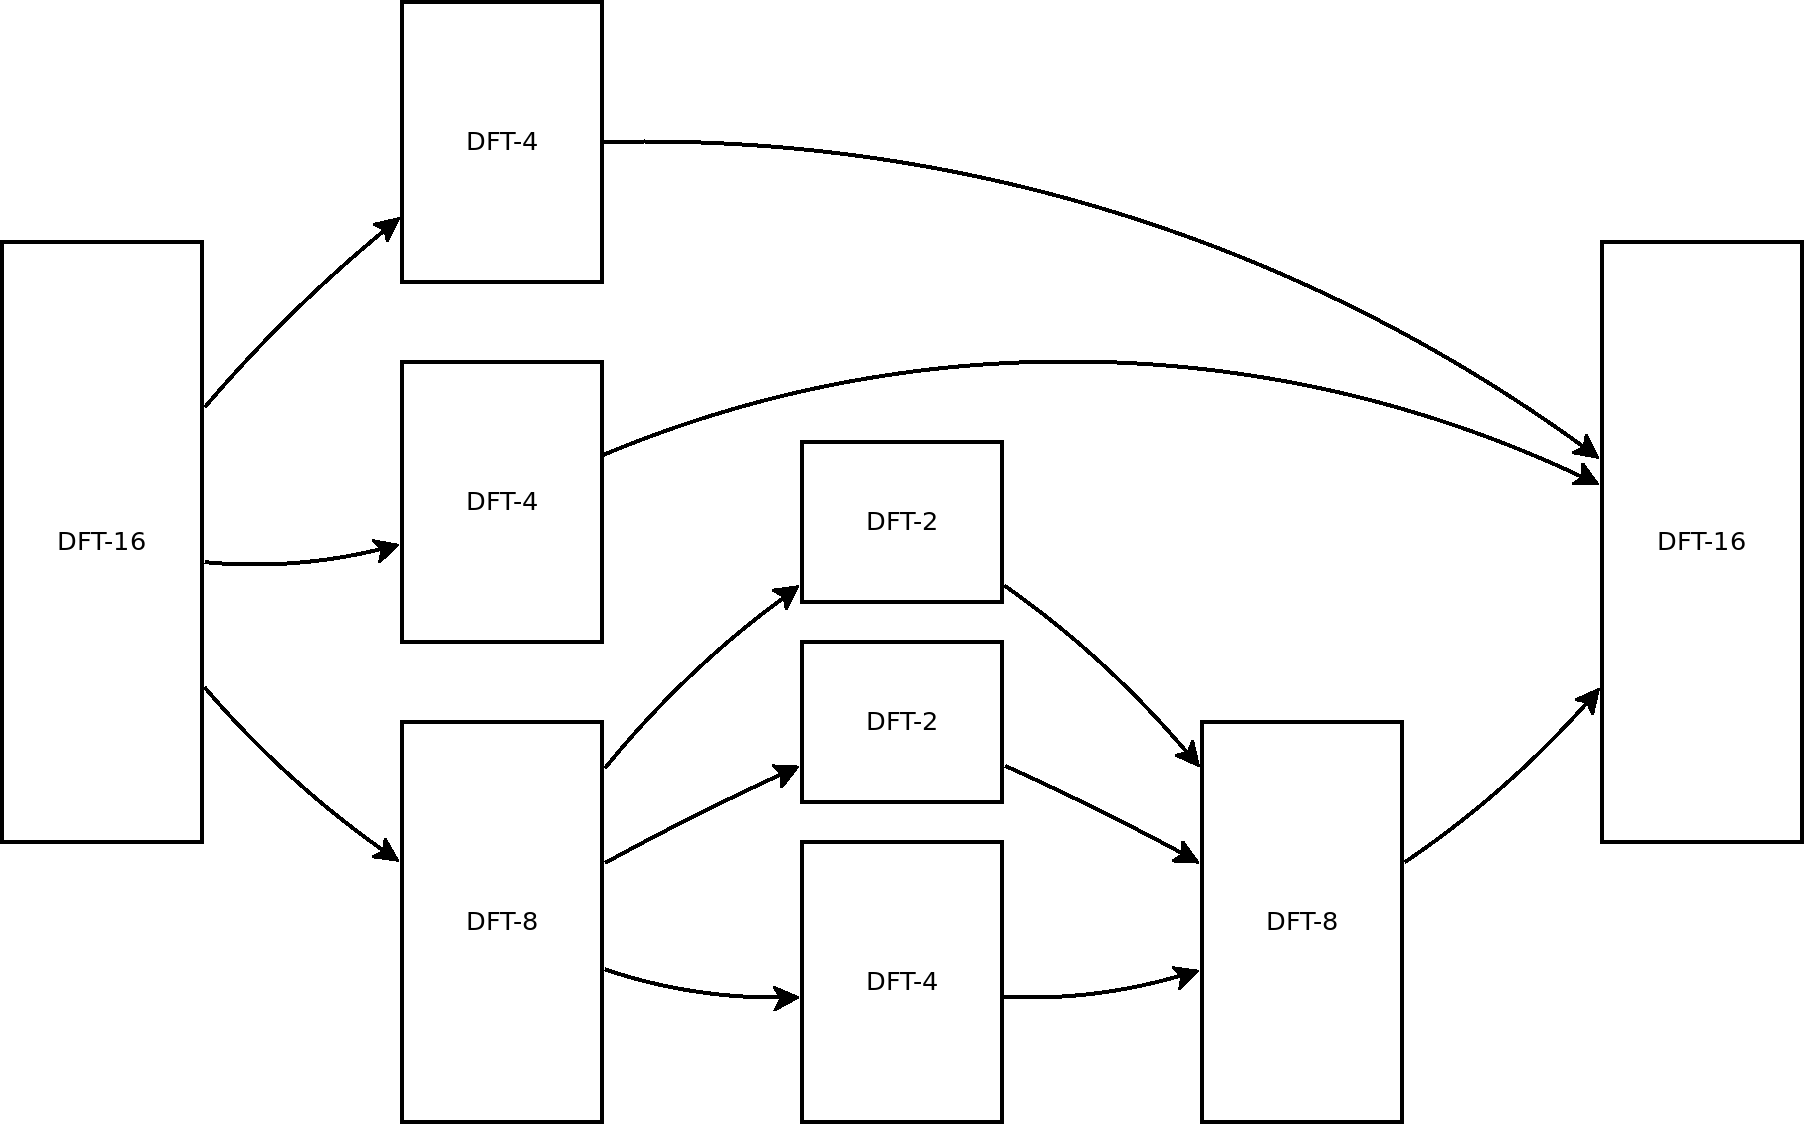
\includegraphics[scale=0.15]{/home/sleepwalking/Documents/IB-EE-FFT/dia/divide-and-conquer-sprdx.png}
		\caption{the divide-and-conquer nature of Split Radix FFT}
	\end{figure}

\section{Mathematical Derivation} \indent

	The following is derivation of Decimation-In-Time(DIT) Split Radix FFT as a background for the next chapter. Another form of Split Radix FFT is Decimation-In-Frequency(DIF). Their differences will be explained in section 2.3.2.
	
	This section is a summary of the reference articles \cite{1984split} and \cite{douglas}.

\subsection{Decimation In Time} \indent

	To simplify the formula, we define a twiddle factor $W_N$ as
	
	\[W_N = e^{-j\frac{2\pi}{N}}\]
	
	where subscript $N$ is the denominator of the exponent, so 
	
	\[W_{N/2} = e^{-j\frac{4\pi}{N}} \quad W_{N/4} = e^{-j\frac{8\pi}{N}}\]

	The DFT formula can be represented with a twiddle factor:
	
	\[X_k = \sum^{N-1}_{n=0} x_n W_N^{nk}\]

	Extract the summation of even indices and two forms of odd indices:
	
	\[X_k = \underbrace{\sum^{N/2-1}_{n=0} x_{2n} W_{N}^{2nk}}_a
	      + \underbrace{\sum^{N/4-1}_{n=0} x_{4n+1} W_{N}^{(4n+1)k}}_b
	      + \underbrace{\sum^{N/4-1}_{n=0} x_{4n+3} W_{N}^{(4n+3)k}}_c\]

	Part a can be rearranged as,
	
	\[\sum^{N/2-1}_{n=0} x_{2n} W_{N}^{2nk} = \sum^{N/2-1}_{n=0} x_{2n} W_{N/2}^{nk}\]
	
	For part b,
	
	\[\sum^{N/4-1}_{n=0} x_{4n+1} W_{N}^{(4n+1)k}
	= \sum^{N/4-1}_{n=0} x_{4n+1} W_{N}^{4nk} \, W_{N}^{k}
	= W_{N}^{k}\sum^{N/4-1}_{n=0} x_{4n+1} W_{N/4}^{nk}\]
	
	The same method applies for part c,
	
	\[\sum^{N/4-1}_{n=0} x_{4n+3} W_{N}^{(4n+3)k}
	= \sum^{N/4-1}_{n=0} x_{4n+3} W_{N}^{4nk} \, W_{N}^{3k}
	= W_{N}^{3k}\sum^{N/4-1}_{n=0} x_{4n+3} W_{N/4}^{nk}\]
	
	Combine the parts together,
	
	\[X_k = \underbrace{\sum_{n=0}^{N/2-1} x_{2n} W_{N/2}^{nk}}_{\text{DFT}\{x_{2n}\}}
          + W_N^k \underbrace{\sum_{n=0}^{N/4-1} x_{4n+1} W_{N/4}^{nk}}_{\text{DFT}\{x_{4n+1}\}}
          + W_N^{3k} \underbrace{\sum_{n=0}^{N/4-1} x_{4n+3} W_{N/4}^{nk}}_{\text{DFT}\{x_{4n+3}\}}\]
	
	So the N-sized DFT is splited to one $\frac{N}{2}$ and two $\frac{N}{4}$-sized DFTs. However, index k is bounded between 0 and $\frac{N}{4}-1$.

\subsection{Expand the Bound} \indent

	The above formula only gives the result when k is bounded between 0 and $\frac{N}{4}-1$ because when $k \geq \frac{N}{4}$, part b and part c are no longer DFTs. To yield a more general result, different ranges of k are discussed respectively.

\subsubsection{Range $k \in [\frac{N}{4}, \frac{N}{2}[$} \indent

	We use $p = k - \frac{N}{4}$ to replace k; the twiddle factors in each sub-DFT remain unchanged:
	
	\[\begin{split}
	W_{N/4}^{n(p+N/4)} & = e^{-j\frac{2\pi}{N/4}n(p+N/4)} \\
					   & = e^{-j\frac{2\pi}{N/4}np} \underbrace{e^{-j\frac{2\pi}{N/4}n(N/4)}}_{= e^{-j2\pi n} = 1} \\
					   & = e^{-j\frac{2\pi}{N/4}np} = W_{N/4}^{np}
	\end{split}\]

	But the twiddle factors outside of sub-DFTs of part b and part c changed:

	\[\begin{split}
	W_N^{p+N/4} & = e^{-j\frac{2\pi}{N}(p+N/4)} \\
				& = e^{-j\frac{2\pi}{N}p} \underbrace{e^{-j\frac{2\pi}{N}(N/4)}}_{= e^{-j\frac{\pi}{2}} = -j} \\
				& = -j W_{N}^p \\
 W_N^{3(p+N/4)} & = W_N^{3p} W_N^{3N/4} = j W_N^{3p}
	\end{split}\]

\subsubsection{Range $k \in [\frac{N}{2}, \frac{3N}{4}[$} \indent

	We use $p = k - \frac{N}{2}$ to replace k and use the same method as above,
	
	\[\begin{split}
	W_{N/4}^{n(p+N/2)} & = W_{N/4}^{np} \\
	       W_N^{p+N/2} & = -W_N^p \\
	    W_N^{3(p+N/2)} & = W_N^{3p} W_N^{3N/2} = -W_N^{3p}
	\end{split}\]
	
\subsubsection{Range $k \in [\frac{3N}{4}, N[$} \indent

	We use $p = k - \frac{3N}{4}$ to replace k and use the same method as above,
	
	\[\begin{split}
	W_{N/4}^{n(p+3N/4)} & = W_{N/4}^{np} \\
	       W_N^{p+3N/4} & = W_N^{p+N/2} W_N^{N/4} = W_N^{p+N/4} = j W_{N}^p\\
	    W_N^{3(p+3N/4)} & = W_N^{3p} W_N^{3N/4} W_N^{3N/2} = -j W_N^{3p}
	\end{split}\]
	
\subsubsection{The Split Radix} \indent

	The whole algorithm can be represented in a cascaded multi-level split structure. Each split is based on the result of splits in the lower level.
	
	\bigskip
	
	We define $X_1$ as $DFT\{x_{2n}\}$; $X_2$ as $DFT\{x_{4n+1}\}$; $X_3$ as $DFT\{x_{4n+3}\}$.

	\bigskip
	
	For $k \in [0, \frac{N}{4}[$,
	
	\[\begin{split}
  X_k & = X_{1_k} + W_N^k X_{2_k} + W_N^{3k} X_{3_k}\\
  X_{k + N/4} & = X_{1_{k + N/4}} - jW_N^k X_{2_k} + jW_N^{3k} X_{3_k} \\
  X_{k + N/2} & = X_{1_k} - W_N^k X_{2_k} - W_N^{3k} X_{3_k} \\
  X_{k + 3N/4} & = X_{1_{k + N/4}} + jW_N^k X_{2_k} - jW_N^{3k} X_{3_k} \\
	\end{split}\]

\subsection{A Procedural Approach} \indent

	To give an intuition of what exactly the Split Radix algorithm does, we take a transform size N = 16 into the formula and get the following procedure for spliting:
	
	\begin{enumerate}
	\item $DFT_{16}\{x_n\}$ is splited into $DFT_{8}\{x_{2n}\}$, $DFT_{4}\{x_{4n+1}\}$, and $DFT_{4}\{x_{4n+3}\}$.
	\item $DFT_{8}\{x_{2n}\}$ is splited into $DFT_{4}\{x_{4n}\}$, $DFT_{2}\{x_{8n+2}\}$, and $DFT_{2}\{x_{8n+6}\}$.
	\item $DFT_{4}\{x_{4n+1}\}$ is splited into $DFT_{2}\{x_{8n+1}\}$, $x_5$, and $x_{13}$.
	\item $DFT_{4}\{x_{4n+3}\}$ is splited into $DFT_{2}\{x_{8n+3}\}$, $x_7$, and $x_{15}$.
	\item $DFT_{4}\{x_{4n}\}$ is splited into $DFT_{2}\{x_{8n}\}$, $x_4$, and $x_{12}$.
	\item 2-sized DFTs cannot be splited further by Split Radix but can still be splited by DFT:
	\item $DFT_{2}\{x_{8n+2}\}$ can be merged from $x_2$ and $x_{10}$.
	\item $DFT_{2}\{x_{8n+6}\}$ can be merged from $x_6$ and $x_{14}$.
	\item $DFT_{2}\{x_{8n+1}\}$ can be merged from $x_1$ and $x_{9}$.
	\item $DFT_{2}\{x_{8n+3}\}$ can be merged from $x_3$ and $x_{11}$.
	\item $DFT_{2}\{x_{8n}\}$ can be merged from $x_0$ and $x_{8}$.
	\end{enumerate}
	
	The computing procedure is exactly the reverse of the above process. The following diagram visualizes such process with blocks representing merges.

\begin{figure}[htp]
\centering
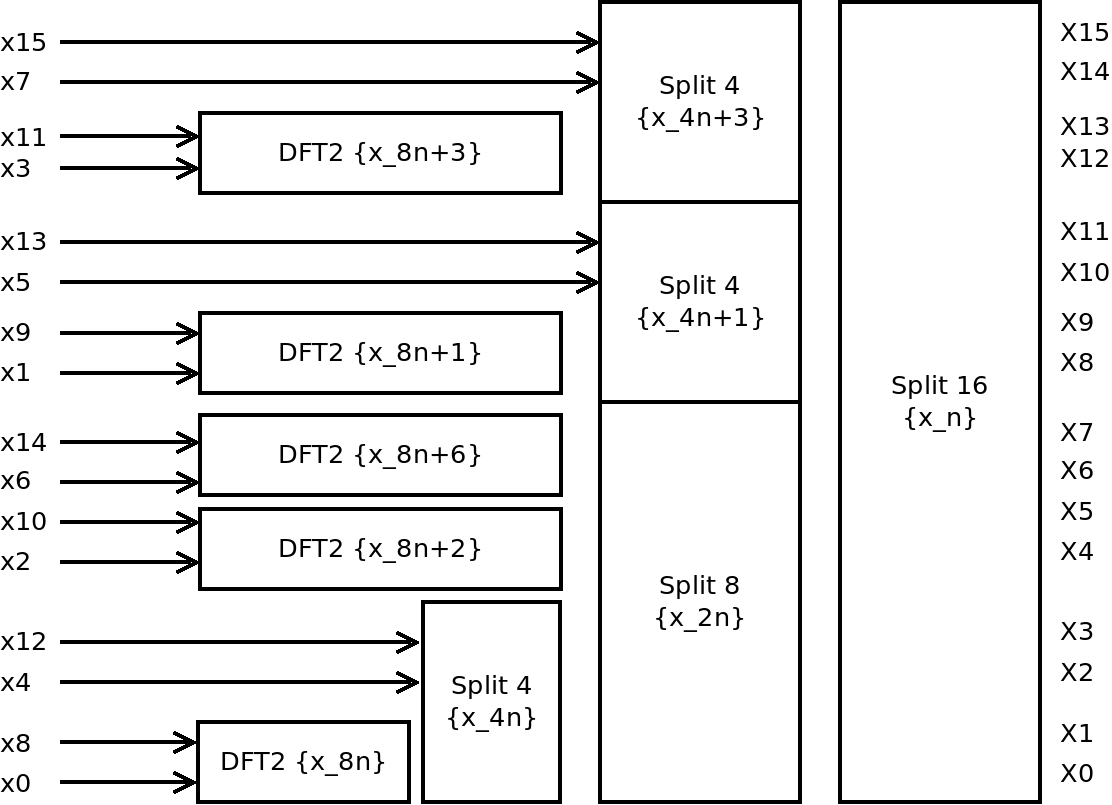
\includegraphics[scale=0.3]{../dia/split-radix-16.png}
\caption{Split Radix Block Diagram, N=16}
\end{figure}

	We can observe that the inputs on the left side are not in original order. This is because in each split the odd and even indices are shuffled.
	
	One way to shuffle the inputs is to use bit reverse method. Take transform with N=16 as an example. The shuffled series of indices in the picture, \{0, 9, 4, 12, 2, 10, ..., 7, 15\} can be generated by the following procedure:
	
	\begin{enumerate}
		\item Generate an array of ascending integers from 0 to $N-1$.
		\item Convert all elements of the array into binary integer each containing $log_2n$ bits. The empty bits are filled with zero.
		\item Reverse the binary integers. For example, 000110 is reversed as 011000.
		\item Convert the binary integers back into decimal integers.
	\end{enumerate}

\section{Points to Consider} \indent

	Before coding, some details have to be considered to trade off between performance and features.

\subsection{Transform Dimension and Precision} \indent

	One dimensional DFT is the most commonly used type of Fourier Transform in Engineering; multi dimensional DFT can be decomposed to cascaded one dimensional transforms. So I will only implement one dimensional FFT.
	
	The need for precision depends on the specific application of FFT. To maximize speed, only single precision floating point type will be involved.

\subsection{DIT v.s. DIF} \indent

	Decimation-In-Frequency FFT, in contrast, splits the transform from the right, i.e., the output side. The derivation method is generally same. Another difference is, the input is ordered but the output is out of order and has to be bit reversed.
	
	The total number of additions and multiplications for DIT and DIF are same. So I just arbitrarily chose DIT.

\subsection{In-place v.s. Out-of-place} \indent

	In-place means the memory region for input is refilled by output after transformation; out-of-place means the output is dumped into another region of memory.
	
\subsubsection{Is it possible to do the whole transform in-place?} \indent

	The answer is true.
	
	\bigskip
	
	Merging the right hand side of the generalized Split Radix formula(see section 2.2.2) gives,
	
	\[\begin{split}
  X_k 		  & = X_{1_k} + \left(W_N^{3k} X_{3_k} + W_N^k X_{2_k}\right)\\
  X_{k + N/4}  & = X_{1_{k + N/4}} + j\left(W_N^{3k} X_{3_k} - W_N^k X_{2_k}\right) \\
  X_{k + N/2}  & = X_{1_k} - \left(W_N^{3k} X_{3_k} + W_N^k X_{2_k}\right) \\
  X_{k + 3N/4} & = X_{1_{k + N/4}} - j\left(W_N^{3k} X_{3_k} - W_N^k X_{2_k}\right) \\
	\end{split}\]
	
	We observe that $X_1$ is copied into $X_k$ and $X_{k + N/2}$. Then addition/subtraction/multiplication with twiddle factors and imaginary unit of $X_3$ and $X_2$ are added onto $X_1$. Such procedure can be implemented in a for-loop without allocating memory for intermediate results.
	
	The following diagram, named as the ``Butterfly Diagram" for its shape similarity, shows the arithmetic procedure of a split. Each arrow denotes an addition and each label above the lines denotes an multiplication.
	
	\begin{figure}[htp]
		\centering
		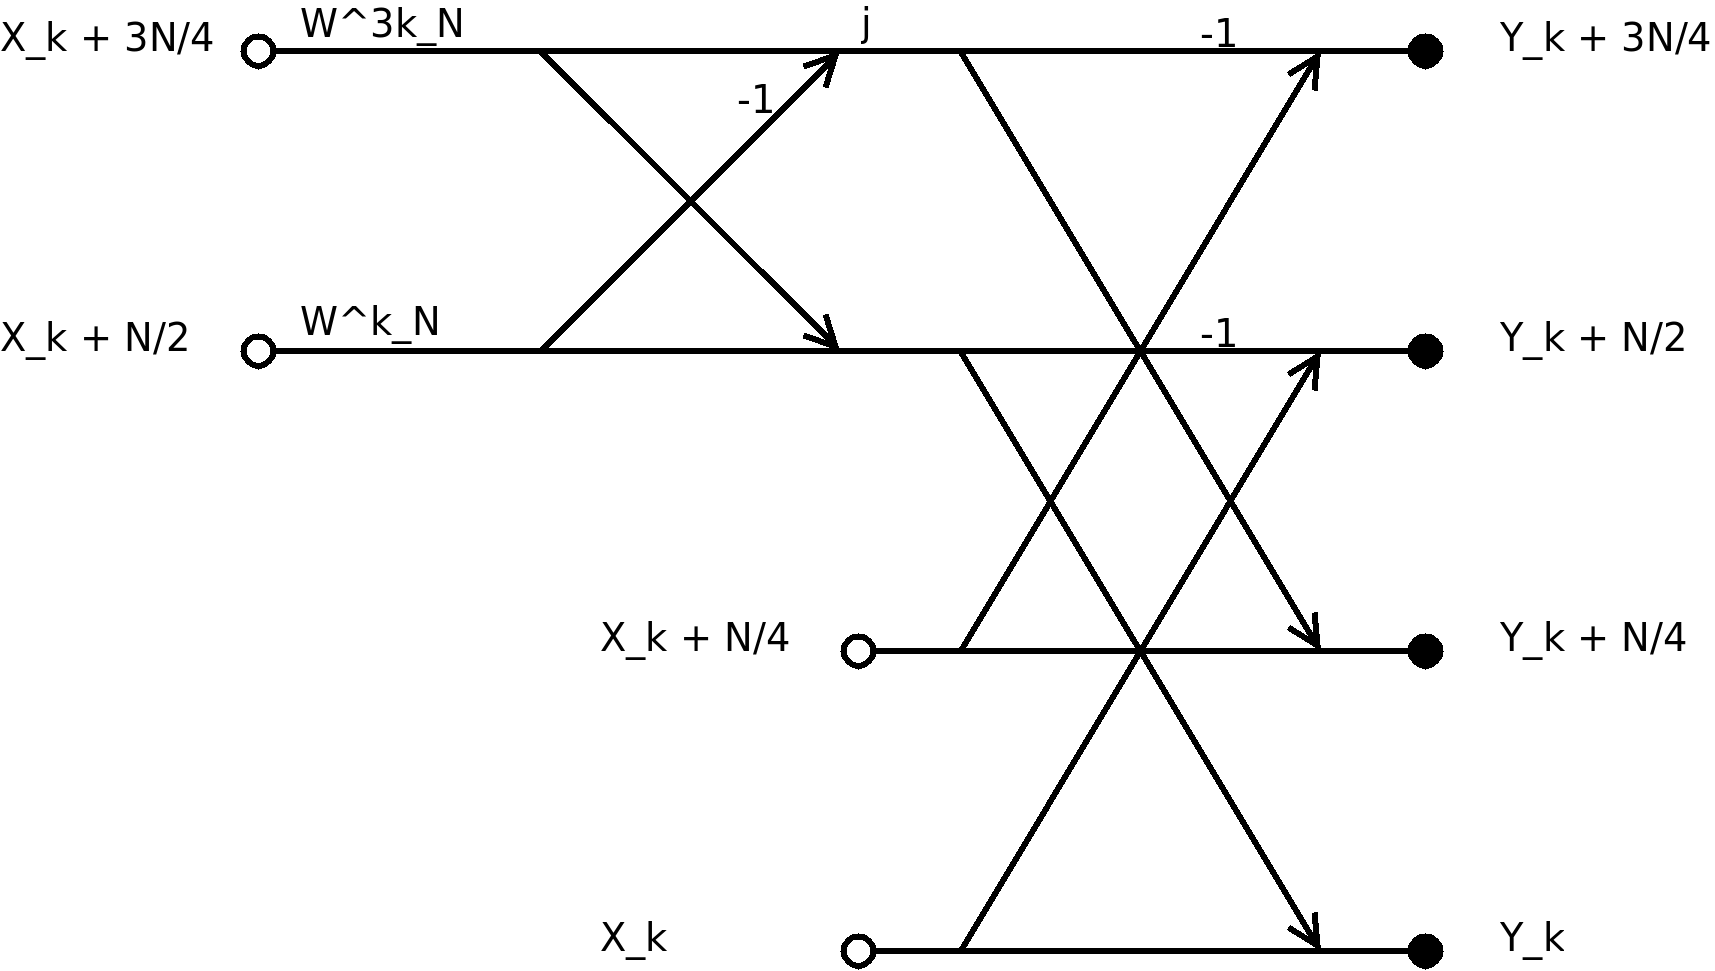
\includegraphics[scale=0.13]{../dia/split-butterfly.png}
		\caption{Split Radix Butterfly Structure}
	\end{figure}

\newpage

	By the way, the above diagram also looks like an inverted letter ``L", so the split process is also called L-shaped transform.

\subsubsection{Advantage of In-place transform} \indent

	Since no extra memory has to be allocated to store intermediate results, the in-place transform makes better use of data cache.

\subsubsection{Disadvantage of In-place transform} \indent

	The input may not be aligned to 16-byte boundaries. So in-place transform can incur a delay in data fetch and storage.

\subsubsection{A Compromise} \indent

	The bit reverse procedure should be out-of-place to shuffle the unaligned inputs into an aligned buffer. After transform the output is copied from the aligned buffer to the unaligned destination.

\subsection{AoS v.s. SoA} \indent

	AoS and SoA are respectively the abbreviations for ``Array of Structure" and ``Structure of Array".
	
	Both the input and output of DFT are complex values. So the AoS solution is to store them as a two dimensional array, of which the first dimension of index of signal, the second is real and imaginary part. The SoA solution involves two one dimensional arrays, one contains all real values, the other contains all imaginary values.

	When doing SIMD optimization on AoS data, we have to do lots of shuffles on data, which can be rather complicated. So I chose SoA for simplicity.
	
\subsection{Choosing the Base Transform} \indent

	In section 2.2.3 the minimal transform is 2-point DFT. If we set N=2, the DFT formula can be simplified as:

\begin{align*}
	X_k &= \sum^{1}_{n=0} x_n e^{-j\frac{2\pi}{N}nk}, \quad k = 0, 1 \\
	X_0 &= x_0 + x_1 \\
	X_1 &= x_0 - x_1
\end{align*}

	which is the sum and difference of two inputs.
	
	\bigskip
	
	Actually in 4-point DFT transforms, there is also no multiplication required:

\[X_k = \sum_{n=0}^{3} x_n e^{-j\frac{2\pi}{4}nk} = \sum_{n=0}^{3} x_n e^{-j\frac{\pi}{2}nk} \]

\begin{align*}
X_0 &= \sum_{n=0}^{3} x_n = x_0 + x_1 + x_2 + x_3 \\
X_1 &= \sum_{n=0}^{3} x_n e^{-j\frac{\pi}{2}n} = x_0 - jx_1 - x_2 + jx_3 \\
X_2 &= \sum_{n=0}^{3} x_n e^{-j\pi n} = x_0 - x_1 + x_2 - x_3 \\
X_3 &= \sum_{n=0}^{3} x_n e^{-j\frac{3\pi}{2} n} = x_0 + jx_1 - x_2 - jx_3
\end{align*}

	We need to pay attention that the input for above process are not bit reversed. So the 4-point transform should be changed as:
	
\begin{align*}
X_0 &= \sum_{n=0}^{3} x_n = x_0 + x_2 + x_1 + x_3 \\
X_1 &= \sum_{n=0}^{3} x_n e^{-j\frac{\pi}{2}n} = x_0 - jx_2 - x_1 + jx_3 \\
X_2 &= \sum_{n=0}^{3} x_n e^{-j\pi n} = x_0 - x_2 + x_1 - x_3 \\
X_3 &= \sum_{n=0}^{3} x_n e^{-j\frac{3\pi}{2} n} = x_0 + jx_2 - x_1 - jx_3
\end{align*}

\section{The System Design} \indent

	\textit{ee-fft} will consist of the following modules:
	
	\begin{enumerate}
		\item A bit reverse module to shuffle the inputs and align them in buffers.
		\item 2-point DFT blocks, which are also called Radix-2 blocks.
		\item 4-point DFT blocks, which are also called Radix-4 blocks.
		\item Split blocks for arbitrarily sized(any integer power of 2) transforms.
	\end{enumerate}
	
	For 8-point split process, few multiplications are involved. So these blocks are replaced by specifically optimized Split-8 blocks:

\[\begin{split}
  X_{0} & = X_{1_0} + X_{2_0} + X_{3_0}\\
  X_{1} & = X_{1_1} + W_8 X_{2_1} + W_8^3 X_{3_1}\\
  X_{2} & = X_{1_2} - jX_{2_0} + j X_{3_0}\\
  X_{3} & = X_{1_3} - jW_8 X_{2_1} + jW_8^3 X_{3_1}\\
  X_{4} & = X_{1_0} - X_{2_0} - X_{3_0}\\
  X_{5} & = X_{1_1} - W_8 X_{2_1} - W_8^3 X_{3_1}\\
  X_{6} & = X_{1_2} + jX_{2_0} - jX_{3_0}\\
  X_{7} & = X_{1_3} + jW_8 X_{2_1} - jW_8^3 X_{3_1}\\
\end{split}\]

	Because the control flow of Split Radix FFT is independent from the data flow, i.e., the data doesn't affect the process of calculations, the implementation can be fully unrolled that does not even has a loop. However, as mentioned in section 1.2.2, such unroll increases the instruction cache miss rate. My solution is to pack the unrolled small transforms into functions, and then pack the functions into larger transforms. In such process no conditional branch is added, thus decreases the branch prediction fail rate.

\begin{figure}[htp]
\centering
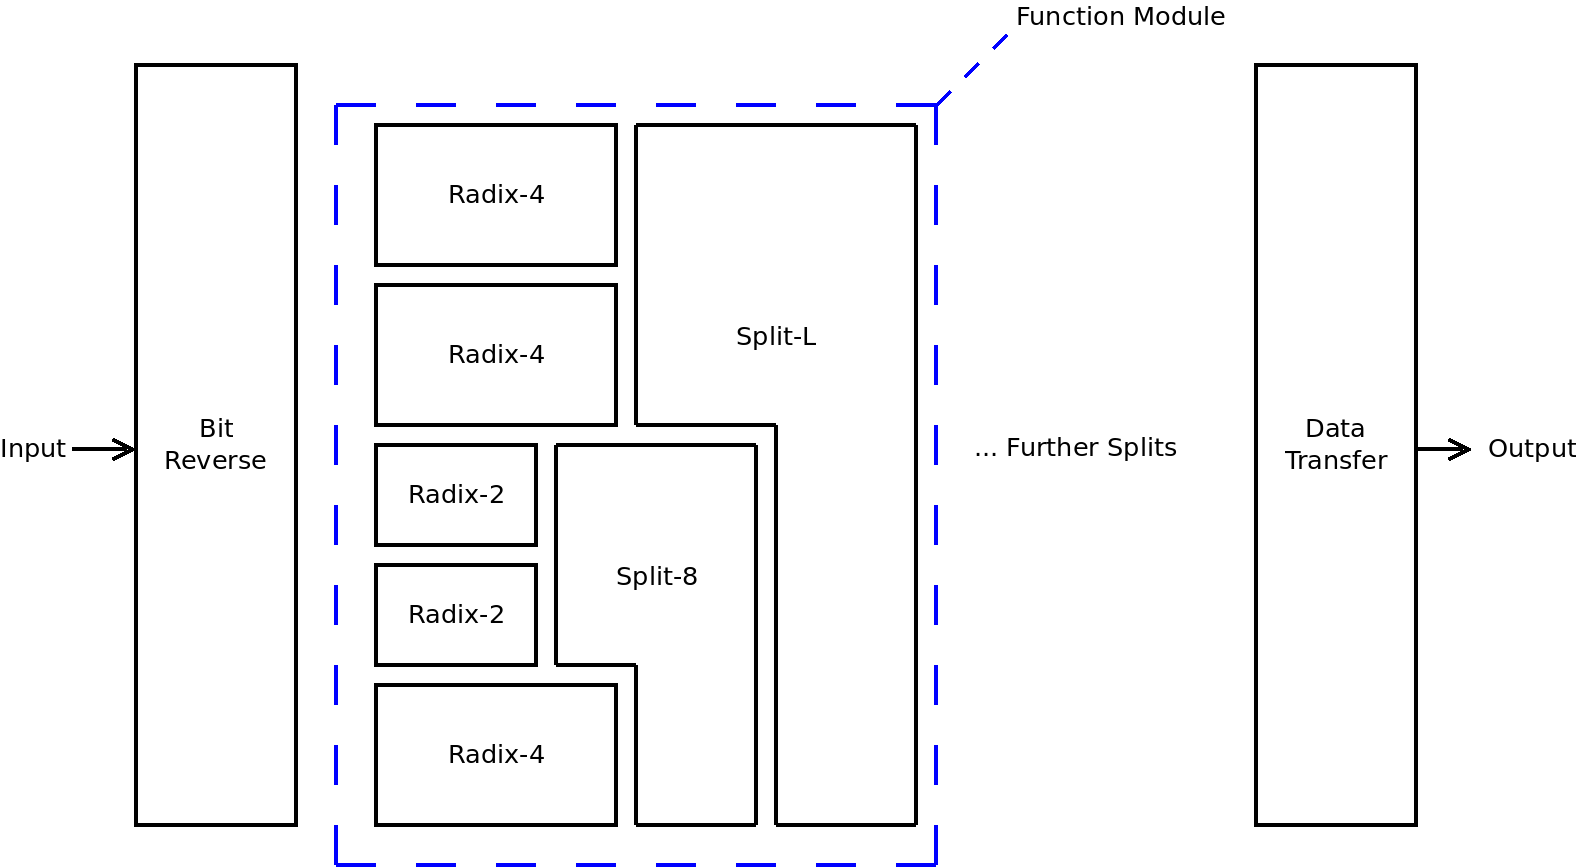
\includegraphics[scale=0.21]{/home/sleepwalking/Documents/IB-EE-FFT/dia/sys-structure.png}
\caption{the overall system structure}
\label{}
\end{figure}
\chapter{The Implementation} \indent

	In this chapter I will present the creation and optimization of each module in the design discussed in section 2.4.
	
	Each section will contain a C implementation and an optimized version using gcc assembly extension. Section 3.6 will discuss about how to assemble \textit{ee-fft} using several established modules.

\section{Bit Reverse Module} \indent

	The bit reverse method has been introduced in section 2.2.3. Since real and imaginary parts are moved together in this process, we can write a out-of-place function that shuffles one portion of the complex numbers and call it twice.
	
\subsection{Bit Reverse in C} \indent

        \lstset{language = c, tabsize = 4}
        \begin{lstlisting}
/* Shuffles the real array src into dst. Power is transform size in power of 2. */
void bitrev(float* dst, float* src, int power)
{
    int N, i, j;
    int tmp = 0x00000000; /* reversed index */
    N = pow(2, power); /* size of data */
    
    /* The first input always corresponds to the first output. */
    dst[0] = src[0];
    for(i = 0; i < N - 1; i ++) /* for each input */
    {
        j = power - 1; /* bit traverse counter */
        
        /* The following code adds an 1 to tmp from the left. */
        while((tmp & (1 << j)) != 0)
        {
            tmp &= ~ (1 << j);
            j --;
        }
        tmp |= (1 << j);
        
        /* shuffle */
        dst[i + 1] = src[tmp];
    }
}
        \end{lstlisting}

\subsection{Static Bit Reverse Generator} \indent

	The above code has lots of branches and loops that cause the program run very slow. One method to optimize this is to fully unroll the loop.
	
	The \textit{bitrev} function's behavior only depends on \textit{Power}. So we can write multiple unrolled functions each corresponds to a certain input of \textit{Power}. The intuition is to write another program that is a ``Code Generator", which outputs the possibly very long and monotone process of unrolled \textit{bitrev} functions for each transform size.
	
	For data transfer of single precision floating point values, SSE instruction \textbf{movss} can be used to replace IA-32 instruction \textbf{mov}. To further optimize, XMM registers are used in circulation:

        \lstset{language = c, tabsize = 4}
        \begin{lstlisting}
    for(i = 0; i < N - 1; i ++)
    {
    	/*
    		codes to generate tmp
    	*/
        printf("\"movss %d%%1, %%%%xmm%d\\n\"\n", tmp * 4, i % 8);
        printf("\"movss %%%%xmm%d, %d%%0\\n\"\n", i % 8, i * 4 + 4);
	}
        \end{lstlisting}

	The complete codes are located at src/gen/genrev.c .
	
	Example of using \textit{genrev} under Unix shell:

        \lstset{language = sh, tabsize = 4}
        \begin{lstlisting}
$ ./genrev -a 2 > bitrev.c
$ cat bitrev.c
static void bitrev_2(float* dst, float* src)
{
    __asm__ __volatile__
    (
        "movss %1, %%xmm0\n"
        "movss %%xmm0, %0\n"
        "movss 8%1, %%xmm0\n"
        "movss %%xmm0, 4%0\n"
        "movss 4%1, %%xmm1\n"
        "movss %%xmm1, 8%0\n"
        "movss 12%1, %%xmm2\n"
        "movss %%xmm2, 12%0\n"
    : "+m"(*dst)
    : "m"(*src)
    : "%xmm0", "%xmm1", "%xmm2", "%xmm3", "%xmm4", "%xmm5", "%xmm6", "%xmm7"
    );
}
        \end{lstlisting}

\section{Radix-2 Block} \indent

	Numerical computation method has been discussed in section 2.3.5.

\subsection{Radix-2 in C} \indent

	This is rather easy:
	
    \lstset{language = c, tabsize = 4}
    \begin{lstlisting}
float tmp_re, tmp_im;
tmp_re = real[0] + real[1];
tmp_im = imag[0] + imag[1];
real[1] = real[0] - real[1];
imag[1] = imag[0] - imag[1];
real[0] = tmp_re;
imag[0] = tmp_im;
    \end{lstlisting}

\subsection{SIMD Optimized Packed Radix-2} \indent

	If the above codes are optimized using SSE instructions, only half of an XMM register can be utilized.
	
	Figure 2.4 in the last chapter shows Radix-2 transforms only directly output to Split-8 transforms. So all Radix-2 blocks appear in pairs, of which input consists of four real successive real values and four successive imaginary values. In other words, Radix-2 blocks can be packed.

	If we use R0, R1, R2... and I0, I1, I2... to denote real and imaginary input/output and left arrow to denote value assignment, the arithmetic flow of packed Radix-2 would be:

\begin{alltt}
\centering
R0 <- R0 + R1
R1 <- R0 - R1
R2 <- R2 + R3
R3 <- R2 - R3

I0 <- I0 + I1
I1 <- I0 - I1
I2 <- I2 + I3
I3 <- I2 - I3
\end{alltt}

	SSE2 instruction \textbf{pshufd} provides a way to shuffle the ordered inputs to arbitrary ordered combination of four. The optimized version in gcc assembly extension is:

    \lstset{language = c, tabsize = 4}
    \begin{lstlisting}
        __asm__ __volatile__
        (
            "movaps %0, %%xmm0                 \n"
            "pshufd $0b11110101, %%xmm0, %%xmm1\n"
            "movaps %1, %%xmm2                 \n"
            "pshufd $0b10100000, %%xmm0, %%xmm0\n"
            "mulps  %%xmm7, %%xmm1             \n"
            "pshufd $0b11110101, %%xmm2, %%xmm3\n"
            "mulps  %%xmm7, %%xmm3             \n"
            "pshufd $0b10100000, %%xmm2, %%xmm2\n"
            "addps  %%xmm1, %%xmm0             \n"
            "movaps %%xmm0, %0                 \n"
            "addps  %%xmm3, %%xmm2             \n"
            "movaps %%xmm2, %1                 \n"
            : "+m"(R), "+m"(I)
            :
            : "%xmm0", "%xmm1", "%xmm2", "%xmm3", "%xmm7"
        );
    \end{lstlisting}
    
    XMM7 should be loaded with a vector \{1.0, - 1.0, 1.0, - 1.0\} before the above process.

\section{Radix-4 Block} \indent

	Numerical computation method has been discussed in section 2.3.5.

\subsection{Radix-4 in C} \indent

    \lstset{language = c, tabsize = 4}
    \begin{lstlisting}
float R0, R1, R2, R3;
float I0, I1, I2, I3;

R0 = real[i];
R1 = real[i+1];
R2 = real[i+2];
R3 = real[i+3];
I0 = imag[i];
I1 = imag[i+1];
I2 = imag[i+2];
I3 = imag[i+3];

real[i  ] = +R0 +R2 +R1 +R3;
real[i+1] = +R0 -R2 +I1 -I3;
real[i+2] = +R0 -R1 +R2 -R3;
real[i+3] = +R0 -R2 +R3 -I1;

imag[i  ] = +I0 +I2 +I1 +I3;
imag[i+1] = +I0 -I2 +R3 -R1;
imag[i+2] = +I0 -I1 +I2 -I3;
imag[i+3] = +I0 -I2 +R1 -I3;
    \end{lstlisting}

\subsection{SIMD Optimized Radix-4} \indent

\subsubsection{Arithmetic Flow} \indent

\begin{alltt}
\centering
R0 <- +R0 +R1 +R2 +R3
R1 <- +R0 -R1 +I2 -I3
R2 <- +R0 +R1 -R2 -R3
R3 <- +R0 -R1 -I2 +I3

I0 <- +I0 +I1 +I2 +I3
I1 <- +I0 -I1 -R2 +R3
I2 <- +I0 +I1 -I2 -I3
I3 <- +I0 -I1 +R2 -R3
\end{alltt}

\subsubsection{The Codes} \indent

    \lstset{language = c, tabsize = 4}
    \begin{lstlisting}
    __asm__ __volatile__
    (
        "movaps %0, %%xmm0\n"                  
        "movaps %1, %%xmm1\n"                  
        "pshufd $0b00000000, %%xmm0, %%xmm2\n" 
        "pshufd $0b01010101, %%xmm0, %%xmm4\n" 
        "pshufd $0b00000000, %%xmm1, %%xmm3\n" 
        "mulps  %3, %%xmm4\n"                  
        "pshufd $0b01010101, %%xmm1, %%xmm5\n" 
        "mulps  %3, %%xmm5\n"                  
        "addps  %%xmm4, %%xmm2\n"              
        "addps  %%xmm5, %%xmm3\n"              
        "punpckhdq %%xmm1, %%xmm0\n"           
        "pshufd $0b01000100, %%xmm0, %%xmm4\n" 
        "pshufd $0b11101110, %%xmm0, %%xmm1\n" 
        "mulps  %2, %%xmm4\n"                  
        "pshufd $0b00111001, %%xmm4, %%xmm5\n" 
        "addps  %%xmm4, %%xmm2\n"              
        "pshufd $0b00010001, %%xmm1, %%xmm4\n" 
        "mulps  %4, %%xmm1\n"                  
        "addps  %%xmm1, %%xmm2\n"              
        "mulps  %2, %%xmm4\n"                  
        "addps  %%xmm5, %%xmm3\n"              
        "addps  %%xmm4, %%xmm3\n"              
        "movaps %%xmm2, %0\n"                  
        "movaps %%xmm3, %1\n"                  
        : "+m"((re)[0]), "+m"((im)[0])         
        : "m"(*NNPP), "m"(*NPNP), "m"(*PNNP)   
        : "%xmm0", "%xmm1", "%xmm2", "%xmm3",  
          "%xmm4", "%xmm5", "%xmm6", "%xmm7"   
    );
    \end{lstlisting}

\subsubsection{Definitions} \indent

	NNPP, NPNP, PNNP are three vectors to store the signs for intermediate computation.

    \lstset{language = c, tabsize = 4}
    \begin{lstlisting}
#define sa16 static __attribute__ ((aligned(16)))
float sa16 NPNP[4] = { 1.0, -1.0,  1.0, -1.0};
float sa16 PNNP[4] = { 1.0, -1.0, -1.0,  1.0};
float sa16 NNPP[4] = { 1.0,  1.0, -1.0, -1.0};
    \end{lstlisting}

\section{Split-8 Block} \indent

	Numerical computation method has been discussed in section 2.4. It can be optimized further in a vector addition form:

\begin{align*}
v_1 &= \{X_{2_0}, W_8 X_{2_1}, -jX_{2_0}, -jW_8 X_{2_1}\}^T\\
v_2 &= \{X_{3_0}, W^3_8 X_{3_1}, jX_{3_0}, jW^3_8 X_{3_1}\}^T
\end{align*}
\begin{align*}
X_{0:3} &= X_1 + v_1 + v_1\\
X_{4:7} &= X_1 - v_1 - v_2
\end{align*}

	Values for twiddle factors involved:

\newcommand{\tsqft}{\frac{\sqrt{2}}{2}}
\[\begin{split}
	W_8 & = e^{-j\frac{2\pi}{8}} = \tsqft - j\tsqft\\
	jW_8 & = je^{-j\frac{2\pi}{8}} = \tsqft + j\tsqft\\
	W^3_8 & = e^{-j\frac{6\pi}{8}} = -\tsqft - j\tsqft = -jW_8\\
	jW^3_8 & = je^{-j\frac{6\pi}{8}} = \tsqft - j\tsqft = W_8
\end{split}\]

\subsection{Arithmetic Flow} \indent

	The input is divided to three parts: 

\begin{itemize}
	\item R0, R1, R2, R3; I0, I1, I2, I3 for $X_1$.
	\item R4, R5; I4, I5 for $X_2$.
	\item R6, R7; I6, I7 for $X_3$.
\end{itemize}

	The sum of $v_1$ and $v_2$, $V$, is computed first, then added to and subtracted from $X_1$.
\begin{alltt}
\centering
n   <- 0.7071067812            \,

VR3 <- -R5*n +I5*n +R7*n +I7*n \,
VR1 <- +R5*n +I5*n -R7*n +I7*n \,
VI3 <- -R5*n -I5*n -R7*n +I7*n \,
VI1 <- -R5*n +I5*n -R7*n -I7*n \,

VR2 <- +I4   -I6               \,
VR0 <- +R4   +R6               \,
VI2 <- -R4   +R6               \,
VI0 <- +I4   +I6               \,

R7  <- +R3 -VR3                \,
R6  <- +R2 -VR2                \,
R5  <- +R1 -VR1                \,
R4  <- +R0 -VR0                \,
R3  <- +R3 +VR3                \,
R2  <- +R2 +VR2                \,
R1  <- +R1 +VR1                \,
R0  <- +R0 +VR0                \,

I7  <- +I3 -VI3                \,
I6  <- +I2 -VI2                \,
I5  <- +I1 -VI1                \,
I4  <- +I0 -VI0                \,
I3  <- +I3 +VI3                \,
I2  <- +I2 +VI2                \,
I1  <- +I1 +VI1                \,
I0  <- +I0 +VI0                \,
\end{alltt}

\subsection{SIMD Optimized Split-8} \indent

    \lstset{language = c, tabsize = 4}
    \begin{lstlisting}
    __asm__ __volatile__
    (
        "movaps %2, %%xmm0                 \n"
        "movaps %3, %%xmm1                 \n"
        "pshufd $0b01010101, %%xmm0, %%xmm2\n"
        "pshufd $0b01010101, %%xmm1, %%xmm3\n"
        "mulps  %4, %%xmm2                 \n"
        "mulps  %5, %%xmm3                 \n"
        "addps  %%xmm3, %%xmm2             \n"
        "pshufd $0b11111111, %%xmm0, %%xmm3\n"
        "pshufd $0b11111111, %%xmm1, %%xmm4\n"
        "mulps  %6, %%xmm3                 \n"
        "mulps  %7, %%xmm4                 \n"
        "addps  %%xmm3, %%xmm2             \n"
        "addps  %%xmm4, %%xmm2             \n"
        "mulps  %8, %%xmm2                 \n"
        "shufps $0b10001000, %%xmm1, %%xmm0\n"
        "pshufd $0b10000010, %%xmm0, %%xmm3\n"
        "pshufd $0b11010111, %%xmm0, %%xmm1\n"
        "mulps  %5, %%xmm3                 \n"
        "mulps  %6, %%xmm1                 \n"
        "subps  %%xmm1, %%xmm3             \n"
        "movaps %%xmm3, %%xmm0             \n"
        "punpckhdq %%xmm2, %%xmm0          \n"
        "punpckldq %%xmm2, %%xmm3          \n"
        "movaps %0, %%xmm1                 \n"
        "movaps %1, %%xmm2                 \n"
        "movaps %%xmm0, %%xmm4             \n"
        "movaps %%xmm3, %%xmm5             \n"
        "addps  %%xmm1, %%xmm4             \n"
        "addps  %%xmm2, %%xmm5             \n"
        "movaps %%xmm4, %0                 \n"
        "movaps %%xmm5, %1                 \n"
        "subps  %%xmm0, %%xmm1             \n"
        "subps  %%xmm3, %%xmm2             \n"
        "movaps %%xmm1, %2                 \n"
        "movaps %%xmm2, %3                 \n"
        : "+m"((re)[0]), "+m"((im)[0]),
          "+m"((re)[4]), "+m"((im)[4])
        : "m"(*NPNN), "m"(*PPNP), "m"(*PNNN), "m"(*PPPN), "m"(*VECN)
        : "%xmm0", "%xmm1", "%xmm2", "%xmm3",
          "%xmm4", "%xmm5", "%xmm6", "%xmm7" 
    );
    \end{lstlisting}

\subsubsection{Definitions} \indent

    \lstset{language = c, tabsize = 4}
    \begin{lstlisting}
#define sa16 static __attribute__ ((aligned(16)))
float sa16 NPNN[4] = {-1.0, -1.0,  1.0, -1.0};
float sa16 PPNP[4] = { 1.0, -1.0,  1.0,  1.0};
float sa16 PNNN[4] = {-1.0, -1.0, -1.0,  1.0};
float sa16 PPPN[4] = {-1.0,  1.0,  1.0,  1.0};
float sa16 VECN[4] = {0.7071067812,  0.7071067812,  0.7071067812,  0.7071067812};
    \end{lstlisting}

\section{L-shaped Split Block} \indent


	Numerical computation method has been shown as the butterfly diagram in section 2.3.3.

\subsection{L-shaped Split Block in C} \indent

	When computing the L-shaped Split, lots of trigonometric functions are called. The C standard library implementation of \textit{sin} and \textit{cos} are extremely slow for numerical computation. To speed up, I used look-up table method, which is to compute the \textit{sin} and \textit{cos} values and store them in large arrays before doing FFT:
	
    \lstset{language = c, tabsize = 4}
    \begin{lstlisting}
static void genw(float* re, float* im, float* re3, float* im3, int N)
{
    int k;
    float omega = 2.0 * M_PI / (float)N;
    
    for(k = 0; k < N / 4; k ++)
    {
        re[k]  = + cos(omega * k);
        im[k]  = - sin(omega * k);
        re3[k] = + cos(omega * k * 3.0);
        im3[k] = - sin(omega * k * 3.0);
    }
}
    \end{lstlisting}
    
    This function is called in \textit{eefft\_init()} to generate look-up tables named in the following format:
    
\begin{alltt}
\centering
w_power_re
w_power_im
w_power_3re
w_power_3im
\end{alltt}
    
    The following code is the C implementation of Split block using look-up table method.

    \lstset{language = c, tabsize = 4}
    \begin{lstlisting}

void split(float* re, float* im, float* w_re, float* w_im,
    float* w_3re, float* w_3im, int N)
{
    int k;
    float* x2_re, *x2_im, *x3_re, *x3_im;
    float tmp_re, tmp_im;
    
    x2_re = re + N / 2;
    x2_im = im + N / 2;
    x3_re = re + 3 * N / 4;
    x3_im = im + 3 * N / 4;
    
    for(k = 0; k < N / 4; k ++)
    {
        //X[k + N/2] <== X[k + N/2] * W_N^k
        tmp_re   = x2_re[k] * w_re[k] - x2_im[k] * w_im[k];
        x2_im[k] = x2_re[k] * w_im[k] + x2_im[k] * w_re[k];
        x2_re[k] = tmp_re;
        
        //X[k + 3N/4] <== X[k + 3N/4] * W_N^{3k}
        tmp_re   = x3_re[k] * w_3re[k] - x3_im[k] * w_3im[k];
        x3_im[k] = x3_re[k] * w_3im[k] + x3_im[k] * w_3re[k];
        x3_re[k] = tmp_re;
        
        //(no dependence)
        //X[k + 3N/4] <== j(X[k + 3N/4] - X[k + N/2])
        //X[k + N/2] <== X[k + N/2] + X[k + 3N/4]
        tmp_re = x3_re[k];
        tmp_im = x3_im[k];
        x3_re[k] = - tmp_im + x2_im[k];
        x3_im[k] = + tmp_re - x2_re[k];
        x2_re[k] += tmp_re;
        x2_im[k] += tmp_im;
    }
    for(k = 0; k < N / 2; k ++)
    {
        tmp_re = re[k];
        tmp_im = im[k];
        re[k] += x2_re[k];
        im[k] += x2_im[k];
        x2_re[k] = tmp_re - x2_re[k];
        x2_im[k] = tmp_im - x2_im[k];
    }
}
    \end{lstlisting}

\subsection{SIMD Optimization with Macros} \indent

	The SIMD optimized version is done in three parts: part A for multiplication with twiddle factors, part B for adding and subtracting on $X_1$, and part C for putting part A and B in for-loops.
	
	Before implementing the parts, a macro \textit{intpow(n)} for ``computing" the integer power of 2 in preprocessing step is written. The code is located at src/module.h .
	
\subsubsection{Part A} \indent

    \lstset{language = c, tabsize = 4}
    \begin{lstlisting}
#define module_splitn_a(re, im, power, _k)\
    __asm__ __volatile__ \
    ( \
        "movaps %0, %%xmm0                 \n" \
        "movaps %1, %%xmm1                 \n" \
        "movaps %%xmm0, %%xmm4             \n" \
        "movaps %%xmm1, %%xmm5             \n" \
        "mulps  %4, %%xmm4                 \n" \
        "mulps  %5, %%xmm5                 \n" \
        "mulps  %4, %%xmm1                 \n" \
        "movaps %2, %%xmm2                 \n" \
        "subps  %%xmm5, %%xmm4             \n" \
        "mulps  %5, %%xmm0                 \n" \
        "movaps %3, %%xmm3                 \n" \
        "addps  %%xmm1, %%xmm0             \n" \
        "movaps %%xmm2, %%xmm1             \n" \
        "mulps  %6, %%xmm1                 \n" \
        "movaps %%xmm3, %%xmm5             \n" \
        "mulps  %7, %%xmm2                 \n" \
        "mulps  %7, %%xmm5                 \n" \
        "subps  %%xmm5, %%xmm1             \n" \
        "mulps  %6, %%xmm3                 \n" \
        "movaps %%xmm0, %%xmm5             \n" \
        "addps  %%xmm3, %%xmm2             \n" \
        "subps  %%xmm2, %%xmm5             \n" \
        "movaps %%xmm1, %%xmm3             \n" \
        "subps  %%xmm4, %%xmm3             \n" \
        "movaps %%xmm5, %2                 \n" \
        "addps  %%xmm1, %%xmm4             \n" \
        "movaps %%xmm3, %3                 \n" \
        "addps  %%xmm2, %%xmm0             \n" \
        "movaps %%xmm4, %0                 \n" \
        "movaps %%xmm0, %1                 \n" \
        : "+m"((re)[intpow(power) / 2 + _k]),     \
          "+m"((im)[intpow(power) / 2 + _k]),     \
          "+m"((re)[intpow(power) / 4 * 3 + _k]), \
          "+m"((im)[intpow(power) / 4 * 3 + _k])  \
        : "m"(w_##power##_re[_k]), "m"(w_##power##_im[_k]),  \
          "m"(w_##power##_3re[_k]), "m"(w_##power##_3im[_k]) \
        : "%xmm0", "%xmm1", "%xmm2", "%xmm3", \
          "%xmm4", "%xmm5", "%xmm6", "%xmm7"  \
    )
    \end{lstlisting}

\subsubsection{Part B} \indent

    \lstset{language = c, tabsize = 4}
    \begin{lstlisting}
#define module_splitn_b(re, im, power) \
    __asm__ __volatile__ \
    ( \
        "movaps %0, %%xmm0                 \n" \
        "movaps %2, %%xmm2                 \n" \
        "movaps %1, %%xmm1                 \n" \
        "movaps %3, %%xmm3                 \n" \
        "addps  %%xmm0, %%xmm2             \n" \
        "addps  %%xmm1, %%xmm3             \n" \
        "subps  %2, %%xmm0                 \n" \
        "subps  %3, %%xmm1                 \n" \
        "movaps %%xmm0, %2                 \n" \
        "movaps %%xmm1, %3                 \n" \
        "movaps %%xmm2, %0                 \n" \
        "movaps %%xmm3, %1                 \n" \
        : "+m"((re)[0]),                 "+m"((im)[0]), \
          "+m"((re)[intpow(power) / 2]), "+m"((im)[intpow(power) / 2]) \
        : \
        : "%xmm0", "%xmm1", "%xmm2", "%xmm3", \
          "%xmm4", "%xmm5", "%xmm6", "%xmm7"  \
    )
    \end{lstlisting}

\subsubsection{Part C} \indent

    \lstset{language = c, tabsize = 4}
    \begin{lstlisting}
#define module_splitn(re, im, power) \
    for(k = 0; k < intpow(power) / 4; k += 4) \
    { \
        module_splitn_a(re, im, power, k); \
    } \
    for(k = 0; k < intpow(power) / 2; k += 4) \
    { \
        module_splitn_b(re + k, im + k, power); \
    } do {} while(0) /* to omit the compiler warning for an extra semicolon */
    \end{lstlisting}
    
\section{Putting the Blocks Together} \indent

	Blocks of \textit{ee-fft} are joined with macros. For example, the following codes build a 8-point fft without bit reverse from Radix-2, Radix-4, and Split-8 blocks:

    \lstset{language = c, tabsize = 4}
    \begin{lstlisting}
#define fft_block_1(re, im) \
    module_radix2(re, im)

#define fft_block_2(re, im) \
    module_radix4(re, im)

#define fft_block_3(re, im) \
    fft_block_1(re + intpow(3) / 2, im + intpow(3) / 2); \
    fft_block_2(re, im); \
    module_split8(re, im)
    \end{lstlisting}

	As mentioned in section 2.4, such complete unroll is bad for cache usage. So after reaching certain size of transform, the block is wrapped in a function:
	
    \lstset{language = c, tabsize = 4}
    \begin{lstlisting}
static void fft_block_5(float* re, float* im)
{
    int k;
    fft_block_3(re + intpow(5) / 2, im + intpow(5) / 2);
    fft_block_3(re + intpow(5) / 4 * 3, im + intpow(5) / 4 * 3);
    fft_block_4(re, im);
    module_splitn(re, im, 5);
}
    \end{lstlisting}
	
	It is found that on most modern processors, wrapping \textit{fft\_block\_5}, \textit{fft\_block\_6}, and \textit{fft\_block\_8} into functions will lead to optimal cache usage for transforms that are equal or less than 2048 points.

\chapter{Evaluation and Review} \indent

	The performance of \textit{ee-fft} and several other FFT packages will be assessed. In the end, some possible ways to further improve \textit{ee-fft} will be pointed out.

\section{Benchmark} \indent

\subsection{Benchmark Method} \indent

	Speeds of different transform size Ns of different FFT packages will be measured. The computation task is to transform 1000 random complex vectors of size N, and repeat such process by 100 times.
	
	The time consumption will be converted to MFLOPS(Million Floating Point Operation Per Second) by the following formula(fftw):
	
	\[\text{MFLOPS} = \frac{5Nlog_2N}{t}\]
	
	Where $t$ is the time for one FFT in milliseconds.
	
	Some FFT packages use AoS data structure as input and output, so a conversion step is necessary before each transform. But the conversion may cause time delay. To be fair, transforms by SoA packages are preceded by a loop that dumps the input to a AoS structure, which will not be actually used by SoA packages.

\subsection{Platforms and Hardwares} \indent

\begin{itemize}
	\item Computer Model: Thinkpad T61
	\item Processor: Intel T7250
	\item Clock Speed: 2GHz
	\item L2 Cache: 2MB
	\item RAM: 1GB
\end{itemize}

\subsection{Softwares} \indent

	Operating System: Debian7.1 32-bit

\subsubsection{FFT Packages} \indent

	All of the following packages are compiled with \texttt{CFLAGS="-msse -msse2 -mno-sse3 -mno-ssse3" FFLAGS="-msse -msse2 -mno-sse3 -mno-ssse3"}.

\begin{itemize}
	\item ee-fft
	\item FFTW 3.3.4, the fastest open source FFT package on most platforms\cite{fftw}.
	\item Ooura FFT, a commonly used FFT package by Takuya Ooura.
	\item Kiss FFT, a small and efficient FFT package.
	\item gsl\_fft, part of GNU Scientific Library(\texttt{gsl\_fft\_complex\_float\_radix2\_forward})
\end{itemize}

\subsection{Benchmark Result} \indent

\begin{figure}[htp]
\centering
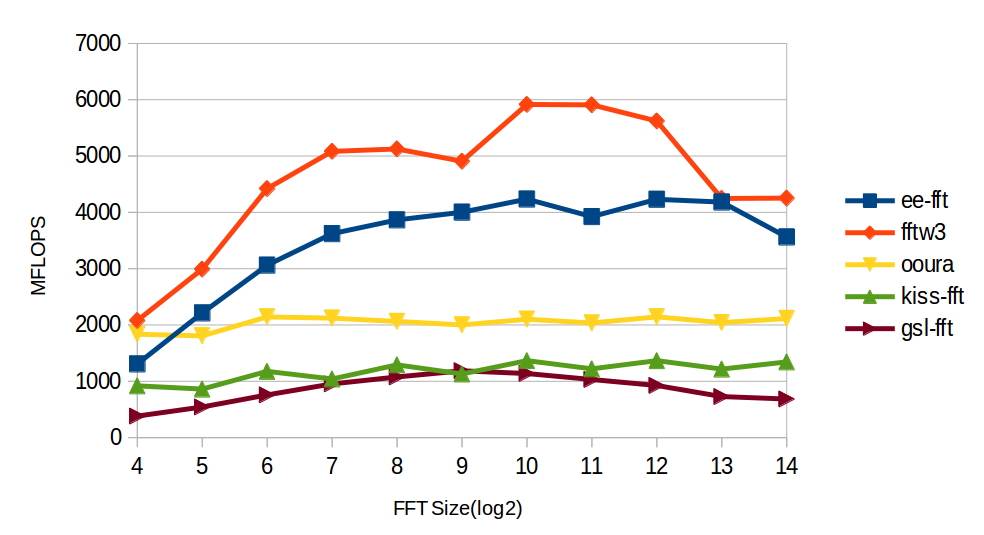
\includegraphics[scale=0.4]{bench.png}
\caption{performance comparison(single thread)}
\end{figure}

	Although \textit{ee-fft} is generally slower than \textit{FFTW3} by $20\%$ to $30\%$, it is much more light-weighted than \textit{FFTW3}. On T61 it takes minutes to compile \textit{FFTW3}, while \textit{ee-fft} takes only three seconds. However, \textit{ee-fft} currently only supports single-precision and single dimensional FFT of integer power of 2 sizes.

\section{Improvements and Extensions} \indent

\subsection{AoS Instead of SoA} \indent

	I observed that most FFT packages use an AoS structure to store inputs and outputs. AoS may be better for data cache usage because real and imaginary parts of a number are packed together instead of stored separately in two arrays.

\subsection{Newer SIMD Instruction Sets} \indent

	SSE3 adds instructions designed for DSP uses and AoS data manipulation; AVX expands the registers to 256 bits and hence can process eight floating point values a time.

\subsection{Porting to Other Platforms} \indent

	Chapter 2 introduces a method to build FFT package by implementing several modules. \textit{ee-fft} can be ported by optimizing these modules for other architectures, for example, ARM, using Neon SIMD instruction set.

\subsection{Alternative Butterfly Structures} \indent

	The reference article\cite{extsplit} presents an alternative Split Radix that decomposes each DFT into a Radix-2 sub transform and a Radix-8 sub transform. It is proved that the extended Split Radix FFT saves 25\% load and store operations.

\appendix

\chapter{Source Code} \indent

	The complete source code of \textit{ee-fft} as well as the \LaTeX \, document of this essay is published in my Github repository:
	
	\bigskip
	https://github.com/Sleepwalking/IB-EE-FFT
	\bigskip

	The essay and diagrams are released under CC-BY-NC-ND 3.0; the source code is released under MIT License.
	
	\bigskip
	
	\textit{gcc} and \textit{cmake 2.8} are required to build \textit{ee-fft}.

\clearpage
\addcontentsline{toc}{chapter}{Bibliography}
\begin{thebibliography}{9}

\bibitem{1984split}
  Duhamel, Pierre and Hollmann, Henk,
  `` `Split radix' FFT algorithm".
  \emph{Electronics Letters},
  vol. 20, pp. 14-16,
  1984.

\bibitem{douglas}
  Jones, Douglas L,
  ``Split-radix FFT algorithms".
  \emph{Connexions web site},
  http://cnx.org/content/m12031/latest/,
  Nov. 2006.

\bibitem{cooley}
  Cooley, James W and Tukey, John W,
  ``An algorithm for the machine calculation of complex Fourier series".
  \emph{Mathematics of Computation},
  vol. 19, pp. 297-301,
  Apr. 1965.

\bibitem{fftw}
  Frigo, Matteo, and Steven G. Johnson,
  ``FFTW: An adaptive software architecture for the FFT".
  \emph{Acoustics, Speech and Signal Processing, IEEE},
  vol. 3, pp. 1381-1384,
  1998.

\bibitem{extsplit}
  Takahashi, Daisuke,
  ``An Extended Split-Radix FFT Algorithm".
  \emph{Signal Processing Letters, IEEE},
  vol. 8, pp. 145-147,
  2001.

\bibitem{inteldev}
  ``Intel 64 and IA-32 Architectures Software Developer’s Manual".
  \emph{Intel, Inc.},
  2013.

\bibitem{intelopt}
  ``Intel 64 and IA-32 Architectures Optimization Reference Manual".
  \emph{Intel, Inc.},
  2013.

\end{thebibliography}
\end{document}
